% ================
% Landon Buell, Kevin Short
% JMM Paper
% PHYS 705.01 - Lab00
% 21 Sept 2020
% ================

\documentclass[conference,onecolumn,letterpaper]{IEEEtran}
%\documentclass[conference,twocolumn,letterpaper]{IEEEtran}

\usepackage{amsmath,amssymb}
\usepackage{graphicx}
\usepackage{float}
\usepackage{cite}
\usepackage{color}
\usepackage{subfigure}
\usepackage[top=2cm,left=1.5cm,right=1.5cm]{geometry}

\usepackage{fancyhdr}
\pagestyle{fancy}
\fancyhf{}
\lhead{Buell, Short}
\rhead{Hybrid Neural Network Classification}
\cfoot{\thepage}

% ================================================================

\title{Musical Instrument Classification Using a Hybrid Neural Network}
\author{Landon H. Buell$^1$ and Kevin M. Short$^2$\\
        $^1$lhb1007@wildcats.unh.edu and 				$^2$kevin.short@unh.edu\\
        $^1$Department of Physics and Astronomy\\
        $^2$Integrated Applied Mathematics Program, Department of Mathematics and Statistics\\
        University of New Hampshire, Durham, New Hampshire, USA\\
       }
        
% ================================================================

\begin{document}

\maketitle

% ================================================================================================================================

\begin{abstract}
    Classifying audio signals with machine learning has become an important topic of research in the past few years. Models often involve the input of a 2-D spectrogram or 1-D feature vector into a unimodal network such as a Convolutional Neural Network (CNN) or Multilayer Perceptron (MLP). In this study, we explore automatic classification of musical instruments using new hybrid neural-network (HNN)  architecture that combines the CNN and MLP models and provides superior performance over models that rely solely on one or the other. This hybrid network uses two branches, one being a CNN to process an image-like 2-D spectrogram, and the other being an MLP to process a 1-D feature vector. Within the model, a hidden layer combines activations from the two branches by concatenating them into a single 1-D dense layer, thus all predictions are a product of both branches. We describe in detail the creating of the spectrogram and features, as well as how they influence the chosen network architecture. We finish with a practical demonstration that uses this classifier model to match waveforms from a chaotic music synthesizer to real-world musical instruments. Training data is from studio recordings of the Philharmonia Symphony Orchestra and University of Iowa's Electronic Music Studios
\end{abstract}

% ================================================================================================================================

\section{Introduction}
\label{sec:Intro}

% ================================================================

Digital audio analysis and classification has become a very active field in the last few years. The exact nature of each task can differ drastically from archival management, to security, or to commercial usage. In each case, we seek to place audio files into distinct categories called \textit{classes} based on inherent properties of the data \cite{James,Khan,Liu}. Consider a collection of audio files, each containing a single note performed by some musical instrument and the task of matching the contents of the file to the instrument that it most closely resembles. This type of classification task is near trivial for humans, but given the terabytes and petabytes of audio data in the modern world, it is impractical at a large scale. However, a computer has no difficulty processing large volumes of raw information, but encoding an explicit and accurate instruction set for classification is unreasonably challenging. For this reason, we turn to a neural network to combine the computational efficiency of a computer, with the decision-making architecture of a simulated brain \cite{Geron}. 

At a basic level, a neural network is a machine learning model that allows a set of inputs, $x$, called \textit{features}, to be transformed into a set of outputs, $y$,  called \textit{predictions} using a set of \textit{parameters}, $\Theta$ \cite{Geron,Goodfellow,Virtanen}. Audio classification with machine learning is also a well-explored field, with much research in developing an appropriate set of features, also called \textit{predictors}, for input \cite{James,Liu,Mierswa,Zhang}. Since the each classification task or data set may differ greatly from any other, each model and data set often requires a unique combination of features which allows for the best possible performance \cite{Virtanen}. For musical instrument classification we have chosen predictors that represent the contents of an audio file using two different \textit{modalities}. We call this type of classification \textit{multimodal learning} \cite{Ngiam}.

Multimodal learning differs from other types of supervised learning in that a model is designed to accept and process multiple inputs simultaneously that are each different representations of the same data sample. Data sets that include or can be transformed into audio + visual, audio + text, or even text + text information, are all examples of multimodal data sets \cite{Li}. For digital audio classification, we have chosen to represent the contents of an audio file by decomposing it into an \textit{image + vector} information format. We do this by constructing a 2D spectrogram and a 1D vector of features from the same waveform. Data from these different modes encodes complementary information which allows a model to develop parameters that can more thoroughly classify a sample when compared to unimodal learning methods \cite{Li}

To accommodate for this multimodal input, we have constructed a \textit{hybrid neural network} (HNN) that utilizes two input branches, each with its own set of layers to handle an input mode. The spectrogram image is processed with a Convolutional Neural Network (CNN) which uses layers of 2D convolution and 2D pooling to generate a feature map, which is then flattened and transformed by repeated dense layers - this is visualized on the left side of Fig. (\ref{fig:Architecture}). The feature vector input is processed by a Multilayer Perceptron (MLP) which uses repeated dense layers to transform the input, and is visualized on the right side of Fig. (\ref{fig:Architecture}). The output of each branch is concatenated into a single layer, which is further transformed into a single output prediction found at the bottom on Fig. (\ref{fig:Architecture}). This means that the neural network learns a set of parameters which allows for mapping of \textit{both} input modes into a single prediction. Since the properties of the input features are critically important to classification success, multi-representation learning shows a great deal of promise and widespread applicability \cite{Khan,Li,Liu,Virtanen}. 

% ================================================================================================================================

\section{The Neural Network}
\label{sec:NeuralNetwork}

% ================================================================

\subsection{Structure}
\label{subsec:Intro}

A neural network defines a type of machine learning algorithm that is inspired from the human brain \cite{Geron,Goodfellow}. Where biological brains are constructed from neurons and connected through axons, neural networks are constructed from artificial neurons and connected through transformation functions. The numerical value contained within an artificial neuron is the \textit{activation} of that neuron \cite{Levine}. Neurons are organized into groups called \textit{layers}, which interact with other layers through mathematical transformations such as matrix multiplications or convolutions \cite{Goodfellow}. Because of this, each layer $l$ in a network can be considered to as function, $f^{(l)}$ that accepts an array of activations from the previous layer $x^{(l-1)}$ and uses a set of parameters to return an array of modified activations for the current layer, $x^{(l)}$. Thus each layer can be generally characterized by the expression:
\begin{equation}
    \label{eqn:LayerFunction}
    f^{(l)} : x^{(l-1)} \rightarrow x^{(l)}
\end{equation}

By connecting multiple layers in succession, we form a layer-chain structure that describes the flow of information in the neural network, and lets us model a neural network as a computational graph \cite{Geron,Goodfellow}. In a feed-forward network with $L$ layers, inputs $x^{(0)}$ and outputs $y^*$, we can represent a layer-chain such as:
\begin{equation}
    \label{eqn:LayerChain}
    x^{(0)} \rightarrow f^{(0)} \rightarrow f^{(1)} \rightarrow ... \rightarrow f^{(L-2)} \rightarrow f^{(L-1)} \rightarrow y^*
\end{equation}
The structure of a neural network's layer-chain defines it's \textit{architecture}. The choice of architecture indicates the \textit{hypothesis-space} of the model a determines the set of all possible solutions that a trained network can attain \cite{Goodfellow,James}. For deep neural networks this function chain can be dozens of layers long, and contain upwards of millions of parameters. Increasingly complicated networks allow for a high dimensional solution space, which potentially enables the modeling of more complex systems.

The hybrid neural network used in this instrument classification task differs from the more standard architecture in Eq. (\ref{eqn:LayerChain}) in that the function chain consists of two input layers, each of which feed into their own respective layer chains, noted by $f_a$ and $f_b$. Each chain transforms activations through a non-overlapping graph, and are then merged at a subsequent hidden layer to produce graph $f_c$. The aggregation of both graphs allows us to generate a single prediction, $y^*$ based on the behavior of both inputs, $x^{(0)}_a$ and $x^{(0)}_b$. We detail the structure an function of each layer chain in section (\ref{subsec:CNN}) and (\ref{subsec:MLP}). We represent the layer-chain structure for a generalized double-input HNN, with inputs $x^{(0)}_a$ and $x^{(0)}_b$ and outputs $y^*$ as :

\begin{equation}
    \label{eqn:LayerGraph}
    \begin{split}
        x^{(0)}_a \rightarrow f^{(0)}_a \rightarrow  ... \rightarrow f^{(\alpha)}_a \searrow &\\
                & f^{(\gamma)}_c \rightarrow ... \rightarrow f^{(L-1)}_c \rightarrow y^* \\
        x^{(0)}_b \rightarrow f^{(0)}_b \rightarrow  ... \rightarrow f^{(\beta)}_b \nearrow &\\
    \end{split}
\end{equation}

This structure allows us to consider and design each branch $a$ and $b$ as if they were separate neural networks. The outputs from $f^{(\alpha)}_a$ and $f^{(\beta)}_b$ can be chosen to represents the predictions of the branches respectively, which are concatenated at layer $f^{(\gamma)}_c$. This marks the entry point of a new chain, which ends at the final output of the full model. Although we may consider the each layer-chain to be it's own entity, it is more appropriate to consider the chains to be subsets of the same computational graph. This means that Eq. (\ref{eqn:LayerGraph}) is considered to be one hybrid neural network model in the training and validation process.

% ================================================================

\subsection{Input and Output}
\label{subsec:InputOutput}

The inputs to a neural network or any machine learning algorithm are called \textit{features} or \textit{predictors} \cite{James}. These are compact, low-dimensional representations of a data sample that reflect its important characteristics \cite{Liu}. Features should be chosen as to have low variance within each class and high variance between classes. For digital audio classification of musical instruments, features of the same musical instruments should exhibit very similar properties, while features from difference musical instruments should exhibit non-similar properties. In any learning algorithm, the role of feature extraction is to translate the raw information from a digital audio file into descriptors that maximize the classification performance \cite{Virtanen}. Although the neural network will classify the musical instrument within the digital audio sample, it will never interact with the raw waveform directly, instead will rely solely on these features. Suppose we implement a classification model that uses $p$ unqiue predictors. These features are usually combined into a single vector-like object for each sample, and then presented as input to the neural network \cite{Geron}. We detail the classification features for this neural network in section (\ref{subsec:FeaturesMLP}) and (\ref{subsec:FeaturesCNN}). 

The outputs to a classification neural network encodes the prediction that the model has made given a particular set of inputs from a sample. For a classifier with $k$ classes, there are $k$ output neurons transformed such that the sum (or $L-1$ norm) of the output activations is identically $1$ \cite{Goodfellow,James}. This means the $k$ neurons can be treated as a probability density for each of the classes, where the neuron with the highest activation value is the prediction of the sample. For classification of musical instruments, each class represents a musical instrument type. We use $37$ classes of instruments encapsulating woodwinds, brass, strings, mallet percussion, and synthesizers. Each audio file contains exactly one musical instrument sustaining one note.

% ================================================================

\subsection{The Cost Function}
\label{subsec:CostFunction}

A neural network is trained by providing a batch of input samples $X$, with a corresponding set of expected predictions $Y$. Consider a sample $x \in X$ that is expected to produce corresponding label $y \in Y$. When passed into the network, $x$ produces some prediction label denoted as $y^*$. For an untrained network, we anticipate that $y^*$ and $y$ may differ greatly - meaning that the prediction is very different that the expected output, and classification performance is likely to be very poor. Since we know each sample in the data set to contain one, and only one musical instrument, we \textit{one-hot-encode} the expected label $y$. For any sample $x^{(i)}$ that belongs to class $j$, we have a corresponding target vector $y^{(i)}$ given by:
\begin{equation}
    \label{eqn:OneHotEnc}
    y^{(i)} = \big[ y_{0} , y_{1}, ... , y_{j}, ... , y_{k-1} \big] = \big[ 0, 0, ... , 1, ... , 0 \big]
\end{equation}
The neural network will output an equivalently sized vector, $y^{*(i)}$, which all elements sum to $1$.

To quantify the difference between $y$ and $y^*$, we introduce a \textit{cost function}, $J(y,y^*)$ which is also called an \textit{objective function} or a \textit{loss function} \cite{James}. The exact cost function used can differ based on the nature of the machine learning model or task, but typically multiple - category classification tasks use a \textit{categorical cross-entropy} (CXE) function \cite{Geron,Goodfellow}. The CXE cost for a single sample is defined as \cite{Goodfellow,Virtanen}:
\begin{equation}
    \label{eqn:CXELoss}
    \text{CXE}[y,y^*] = - \sum_{n=0}^{k-1} y_{n} \ln(y^*_{n})
\end{equation}
Recall a sample belongs to class $j$. Since $y$ is one-hot-encoded, the only non-zero term in the sum is $y_{j} \ln(y^*_{j})$, where $y^*_{j} \in [0,1]$.  This returns a negative number, which we multiply by $-1$ to always yield a positive cost value. When a sample produces $y^*_{j} << 1$, meaning a poor prediction, the CXE cost returns a large value and when $y^*_{j} \approx 1$, meaning a strong prediction, then the CXE cost returns a small value. We provide a visualization of this behavior in Fig. (\ref{fig:CXELoss}).

\begin{figure}[h]
    \centering
    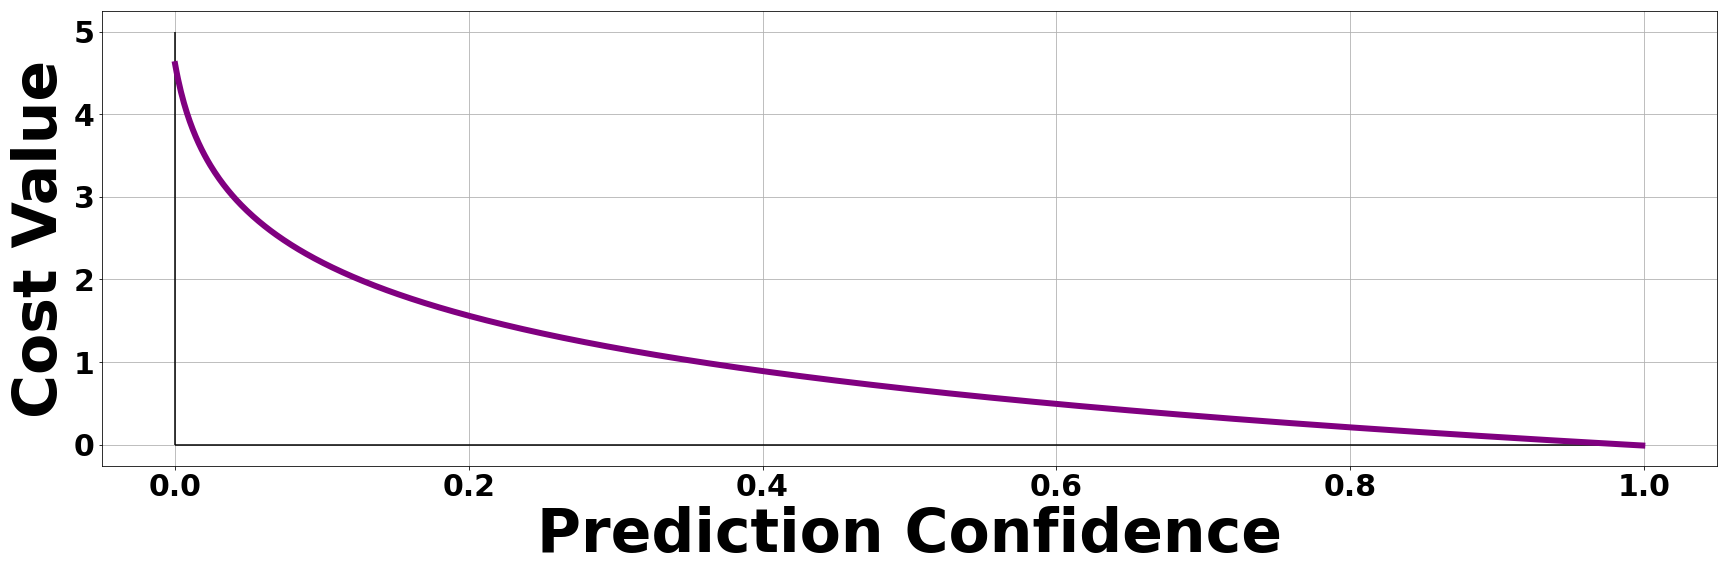
\includegraphics[scale=0.14]{figures/CXELoss.png}
    \caption{Categorical Cross Entropy Cost Function given values for $y^*_{j} \in [0,1]$}
    \label{fig:CXELoss}
\end{figure}

We characterize the cost function as producing a value inversely proportional to the prediction confidence- A large cost value indicates a \textit{poor} prediction label and a low cost value indicates a \textit{strong} prediction label \cite{James,Virtanen}. Thus, we expect a trained neural network to produce consistently low cost function values across all samples in a data set. When a neural network does show this behavior for previously unseen samples, we consider it to be a \textit{fitted} or \textit{trained} neural network \cite{Geron,Goodfellow,James}.

% ================================================================

\subsection{Training and Optimization}
\label{subsec:Training}

A neural network makes predictions by successive transformations of input features through layer functions until a final output array is produced. Each layer $f^{(l)}$, of the model is a function that contains a set of parameters held within arrays $W^{(l)}$ and $b^{(l)}$ that are used to transform activations through the layer chain \cite{Goodfellow}. The process of training the network is the manipulation of these parameters in each layer, such that each input $x$ can produce a output, $y^*$ that is reasonably close to $y$. Since we can quantify the difference between the expected output and the given output with a cost function, we can use this as a metric for measuring how "trained" a model is \cite{James}. Specifically, we train a neural network by \textit{optimizing} the parameters in each layer to allow for this consistently low cost function value \cite{Geron,Goodfellow}. Note that we optimize the cost function under the assumption that doing so will also improve the classification performance. This is called \textit{indirect optimization} \cite{Goodfellow}.

Since a the function chain that comprises a neural network can become exceedingly complicated for deeper and wider networks, producing a single analytical expression for the optimization of every parameter may be either impractical at best or impossible at worst. We instead optimize the network with a numerical iterative method based on \textit{gradient descent} \cite{Geron,Goodfellow}. Gradient descent is the process of (i.) computing the gradient of the cost function with respect to every element in $\Theta$ and (ii.) adjusting each parameter in $\Theta$ according to the elements in that gradient vector, shown in Eq.(\ref{eqn:GradDesc}), often scaled by a \textit{learning rate} $\alpha$. We compute the gradient of the cost function, $\nabla_{\Theta}J$ through a process call \textit{backwards propagation} \cite{Geron}. This algorithms uses the derivative chain-rule from multivariate calculus to begin at the last layer of the network, and work backwards through the layer chain in Eq. (\ref{eqn:LayerChain}) to construct the elements of $\nabla_{\Theta}J$ \cite{Goodfellow,Virtanen}.

\begin{equation}
    \label{eqn:GradDesc}
    \Theta^{(i)} = \Theta^{(i-1)} + (-\alpha)\nabla_{\Theta}J
\end{equation}

Standard gradient descent optimization is cumbersome, prone to numerical errors, and may often become unstable when encountering discontinuities in solution-space \cite{James,Geron}. Because of this, we employ a more robust and aggressive optimization algorithm called \textit{Adaptive-Moments} or ADAM for short. ADAM uses adaptive learning rates, $s^{(i)}$ and $r^{(i)}$, that record and update exponentially decaying averages of past gradients and past squared gradients respectively. The ADAM update is given by Eq. (\ref{eqn:ADAM}).

\begin{equation}
    \label{eqn:ADAM}
        \begin{split}
        s^{(i)} &= \rho_1 s^{(i-1)} + (1 - \rho_1) \nabla_{\Theta} \bar{J}  \\
        r^{(i)} &= \rho_2 r^{(i-1)} + (1 - \rho_2) \Big[ \nabla_{\Theta} \bar{J} \odot \nabla_{\Theta} \bar{J} \Big]  \\
        s'^{(i)} &= \frac{s^{(i)}}{1-\rho_1^i} \\
        r'^{(i)} &= \frac{r^{(i)}}{1-\rho_2^i} \\
        \Theta^{(i)} &= \Theta^{(i-1)} + (-\alpha)\frac{s'^{(i)}}{\sqrt{r'^{(i)}}+\delta} \\
        \end{split}
\end{equation}

ADAM provides a much more powerful and stable optimization algorithm at a higher computational cost \cite{Geron}. Note that the superscript $(i)$ indicates an iteration index where a superscript $i$ is exponentiation. Typically we initialize $\rho_1 = 0.9$, $\rho_2 = 0.999$, and introduce $\delta \approx 10^{-7}$ to avoid possible division of near-zero values \cite{Goodfellow}. All operations in the final three steps are applied element-wise. ADAM has experimentally shown to be a very effective optimizer and useful for a wide range of data sets and architectures which is why we have chosen to implement it for this task \cite{Geron,Goodfellow}.

% ================================================================================================================================

\section{Features and the Hybrid Network}
\label{sec:Features}

The architecture that we have developed for this model incorporates a convolutional neural network (CNN) and a multilayer perceptron (MLP) and is visualized in Fig. (\ref{fig:Architecture}). The later hidden layers of the CNN branch flatten a 2D grid of activations into a 1D vector for each sample and pass it them into it's own MLP. The outputs of each branch are concatenated into a single dense layer, and a new output is drawn from the combined array of activations. We detail the structure and input features of each of the two input branches.

% ================================================================

\subsection{Multilayer Perceptron Features}
\label{subsec:FeaturesMLP}

The features for this branch are derived from the time-domain or frequency-domain representation of a waveform. Each feature explored represents the values computed from each audio file, which are then assembled into a 1D array-like object called a feature vector. This vector is provided as input to the MLP branch of the neural network, which can be found on right side of Fig. (\ref{fig:Architecture}). To ensure a consistency of all extracted features, all waveforms have been truncated or zero-padded to contain a consistent $M$ samples.

\begin{enumerate}

\item\textbf{Time Domain Envelope} (TDE) - 
The TDE is a method of approximating the energy in the full or a subset of the time-series waveform of a signal. We divide the waveform into $5$ non-overlapping analysis frames and compute the RMS energy of the waveform in each section. This allows for an approximation of the amplitude envelope of the time-domain signal \cite{Virtanen}. For a signal $s$, the RMS energy in the $j$-th frame containing $Q$ samples is given by:
\begin{equation}
    \label{eqn:TDE}
    \text{TDE}_j[s] = \sqrt{\frac{1}{Q}\sum_{i=n}^{n+Q}s[i]^2}
\end{equation}
These features allow us to characterize the time-evolution of energy in a signal. Instruments with heavy attacks, and sudden decays show large TDE values in early frames, and low TDE values in later frames. Instruments with longer sustains will show consistently decaying TDE values throughout the duration of the file.

\item\textbf{Zero Crossing Rate} (ZXR) - 
The ZXR of a waveform measures how many time that a signal crosses it's equilibrium value, often normalized per unit time. This feature is commonly used to differentiate speech from music because speech often has a more jagged and less periodic structure, giving it a characteristically higher ZXR value \cite{Virtanen,Khan,Zhang}. We adapt this feature to compute the zero-crossing rate over the full waveform. The zero crossing rate for a waveform $s$ with $M$ samples is given by:
\begin{equation}
    \label{eqn:ZXR}
    \text{ZXR}[s] = \frac{1}{2}\sum_{i=i}^{M-1}\Big| \text{sign}\big(s[i]\big) - \text{sign}\big(s[i-1]\big) \Big|
\end{equation}
Where $\text{sign}(x)$  returns $+1$ if $x > 0$, $-1$ if $x < 0$ and $0$ if $x = 0$. In generally, the zero crossing rate can also be used as a rough frequency measurement, where instruments that can produce higher fundamental frequencies often have higher ZXR values, where instruments that can produce lower fundamental frequencies have lower ZXR values \cite{Zhang}.

\item\textbf{Temporal Center of Mass} (TCM) - 
The TCM of a waveform computes approximately where in time the energy of a waveform is centered around and can conveniently summarize characteristics of the transient response into a single scalar value. The temporal center of mass of a signal $s$ with $M$ samples is given by:
\begin{equation}
    \label{eqn:TCM}
    \text{TCM}[s] = \frac{\sum_{i=0}^{M-1}i\big|s[i]\big|}{\sum_{i=0}^{M-1}\big|s[i]\big|}
\end{equation}
For instruments with heavier attacks and short decay and release times, such as plucked strings or percussion, we expect the energy of the waveform to be very early on, thus providing a very low TCM value. For instruments with shorter attacks, with long sustain and release times, such as bowed strings or woodwinds, we expect the energy of the waveform to be more spread out, thus have a higher TCM value.

\item\textbf{Auto Correlation Coefficients} (ACC) -
ACC's are rough estimates of the signal spectral distribution. They are computed by taking the dot product of a signal with a time-expedited variant of itself, then the normalized to lie between $0$ and $1$ \cite{Virtanen}. We can compute any number of ACC's and it's value will change according to the index chosen. In practice, it is common to compute the first $K$ ACC's, with the $k$-th ACC for a signal $s$, with $M$ samples is given by:
\begin{equation}
    \label{eqn:ACC}
    \text{ACC}_k[s] = \frac{\sum_{i=0}^{M-k-1}s[i]s[i+k]}{\sqrt{\sum_{i=0}^{M-k-1}s^2[i]}\sqrt{\sum_{i=0}^{M-k-1}s^2[i+k]}}
\end{equation}
Dotting this signal with the time-shifted version of itself allows us to measure periodicity in time-space. 

\item\textbf{Mel Frequency Ceptrum Coefficients} (MFCC) - 
In the MFCC computation process, a frequency spectrum is passed through overlapping triangle filter branks that are spaced according to the Mel scale \cite{Sahidullah}. This is done by calculating the dot product between the power spectrum of a signal and each of $R$ Mel filter banks, which yields an approximation of energy in that frequency band. These are called Mel Filter bank energies (MFBE's). Each MFCC is found by computing the inverse discrete cosine transform of the log of the MFBE's. For $R$ filter banks, the $k$-th MFCC is given by \cite{Virtanen}:
\begin{equation}
    \label{eqn:MFCC}
    \text{MFCC}_k[B] = \sqrt{\frac{2}{R}}\sum_{i=1}^{R}\log{(B[i])}
    \cos\Big(\frac{k(i-\frac{1}{2})\pi}{R}\Big)
\end{equation}
Where $B[i]$ is the $i$-th MFBE value. MFCC's allow for the investigation of periodicity in frequency-space, which identifies phenomena of overtones, echoes, etc \cite{Sahidullah,Virtanen}. 

\item\textbf{Frequency Center of Mass} (FCM) - 
FCM computes approximately where in the frequency spectrum, the energy of a waveform is centered around. It is calculated by treating the power spectrum of a signal (or analysis frame) as a 1D discrete mass distribution. The FCM of a power spectrum $\widetilde{s}$, containing $M$ samples is found by:
\begin{equation}
    \label{eqn:FCM}
    \text{FCM}[\widetilde{s}] = 
    \frac{\sum_{i=0}^{M-1}i\big|\widetilde{s}[i]\big|}
    {\sum_{i=0}^{M-1}\big|\widetilde{s}[i]\big|}
\end{equation}
For instruments with lower ranges and fundamental frequencies such as basses, bassoons or cellos, we find a consistently low FCM. For instruments with higher ranges and fundamental frequencies such as flutes, bells, or oboes, we find a consistently large FCM.

\end{enumerate}

Each of these features represents an entry in a $1 \times 24$ \textit{feature-vector} that describes each sample. This object conveys important characterisitcs of each digital audio in a list-like fashion. It is presented as input to the multilayer perceptron branch of the HNN. This is the first of the two modalities that we choose to represent each data sample.

% ================================================================

\subsection{Convolutional Network Features}
\label{subsec:FeaturesCNN}

The features for this branch are the entries in a standard 2D spectrogram representation of a waveform. A spectrogram maps the energy distribution of a signal as a function of time and frequency. It is particularly useful because it allows us to examine the frequency composition of a signal, and how that composition evolves over time. On a typical spectrogram, the passing on time is shown on the x-axis, and frequency is shown on the y-axis. Because it is represented as a 2D array or floating-point numbers, the spectrogram is effectively an image-like representation of a sound wave. Since each musical instrument produces it's own harmonic structure and transient response, each instrument can be identified by patterns within the spectrogram \cite{Virtanen}. This means than when only use this modality, the audio classification becomes very similar to an image classification task \cite{Ngiam}. We provide a few example spectrograms for reference in Fig. (\ref{fig:Example Spectrograms}).

A spectrogram is produced by applying the technique of \textit{frame-blocking} to a waveform to produce a matrix of short-time analysis frames \cite{Liu,Virtanen}. We choose each frame to contain $N = 1024$ samples, with a $768$ sample overlap between adjacent frames. 
\begin{figure}[H]
    \centering
    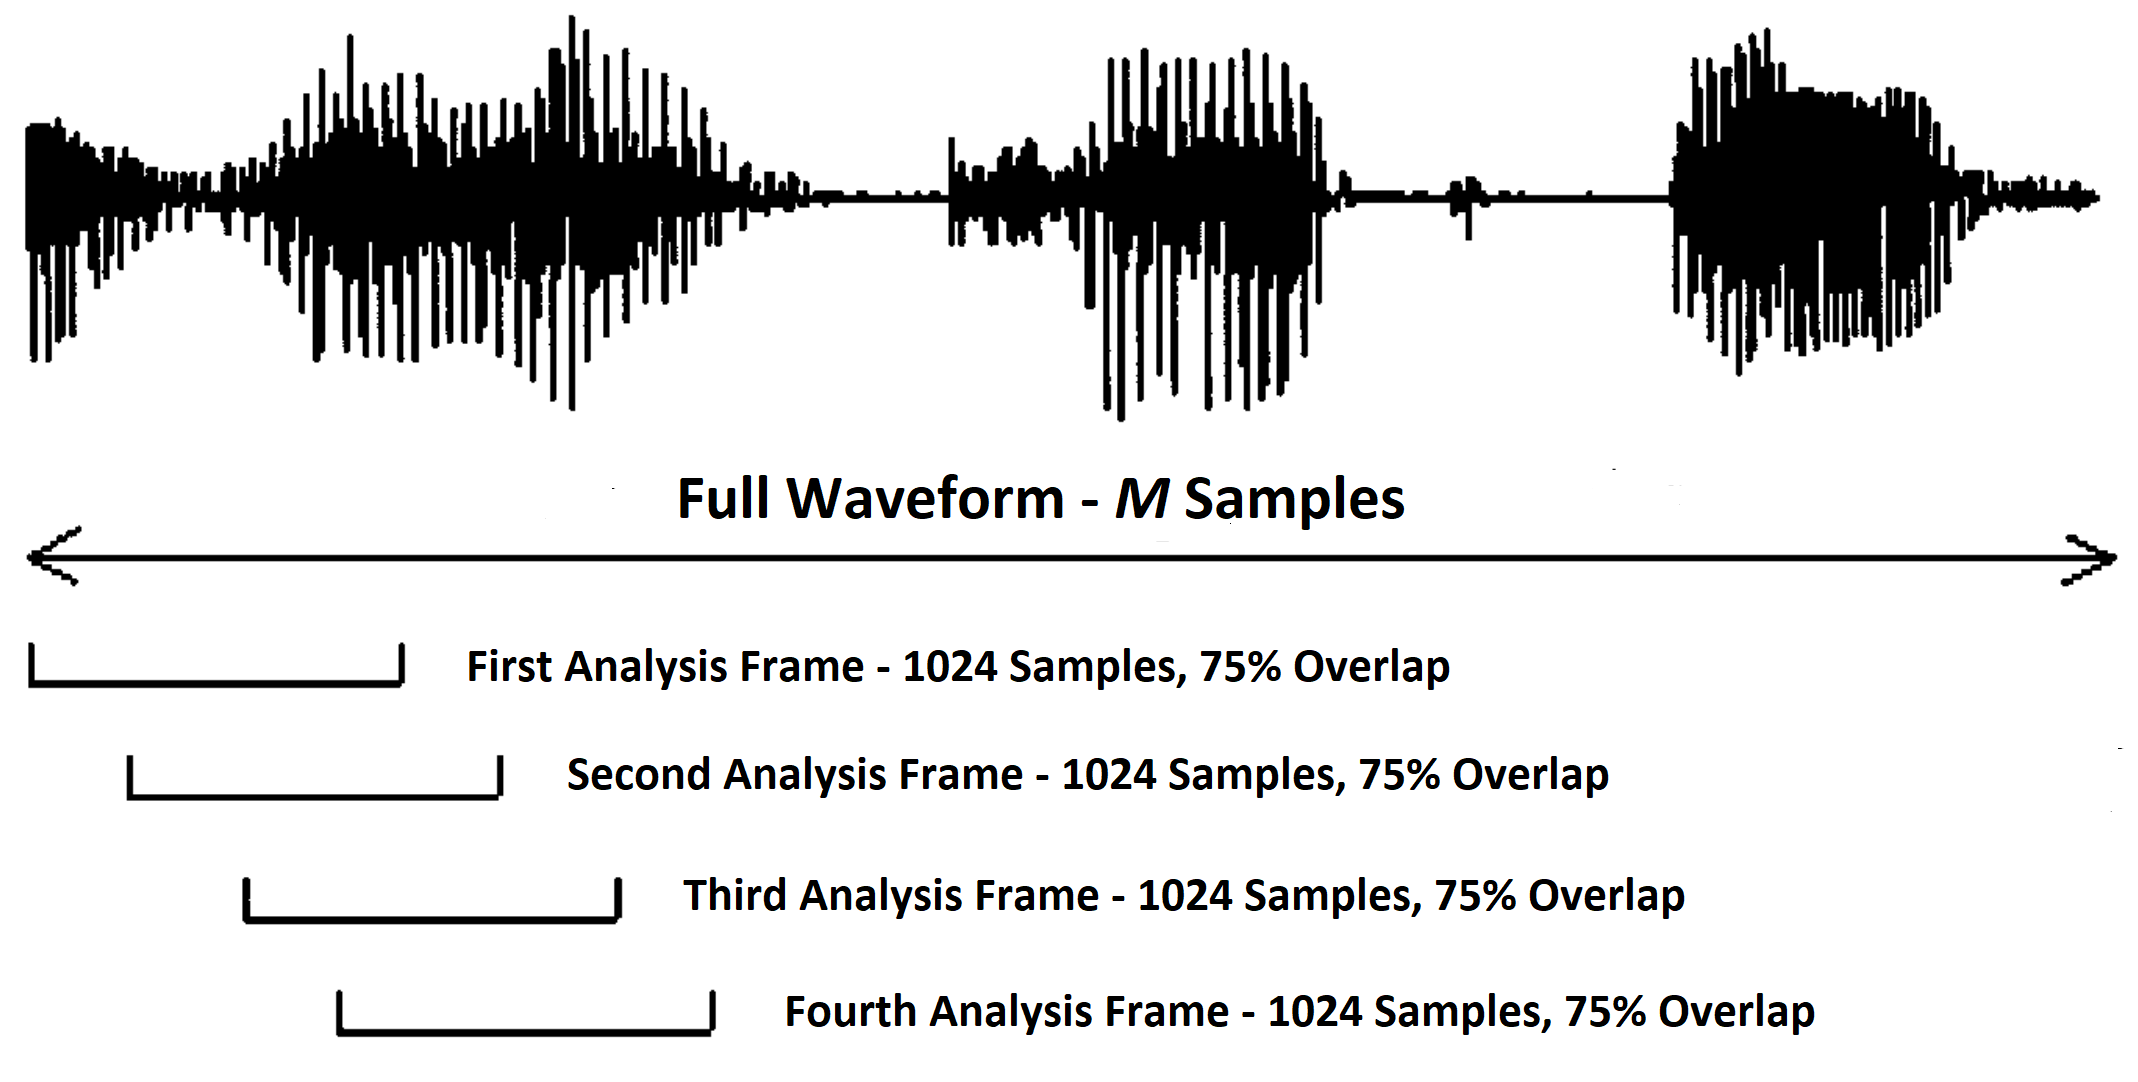
\includegraphics[width=0.45\textwidth]{figures/AnalysisFrames.png}
    \caption{Analysis frames in relation to a full waveform. This figures has been adapted from \cite{Liu}.}
    \label{fig:AnalysisFrames}
\end{figure}
We organize the analysis frames into a matrix, $A$ with shape $N \times k$, such that each row is a frame. We apply a Hanning window of length $N$ to each row of $A$. This eliminates discontinuities at the edges of each analysis frame, and allows for a cleaner transform into frequency-space \cite{Virtanen}. The effect of applying an Hanning window function to an analysis frame of $1024$ samples can be found in Fig. (\ref{fig:WindowFrame}). We tail-pad each time-series analysis frame by an additional $1024$ zeros which brings each frame to $2048$ samples, and gives a higher frequency-space resolution \cite{Sahidullah}. The spectrogram, $S$, is produced by computing:
\begin{equation}
    \label{eqn:Spectrogram}
    S = \big( \mathbb{W}A^T \big) \odot \big( \mathbb{W}A^T \big)^* 
\end{equation}
Where $\mathbb{W}$ is the standard \textit{Discrete Fourier Transform} (DFT) matrix, and $^*$ indicate element-wise complex conjugation. For $k$ analysis frames, matrix $S$ has shape $2048 \times k$. 

\begin{figure}[h]
    \centering
    \subfigure[]{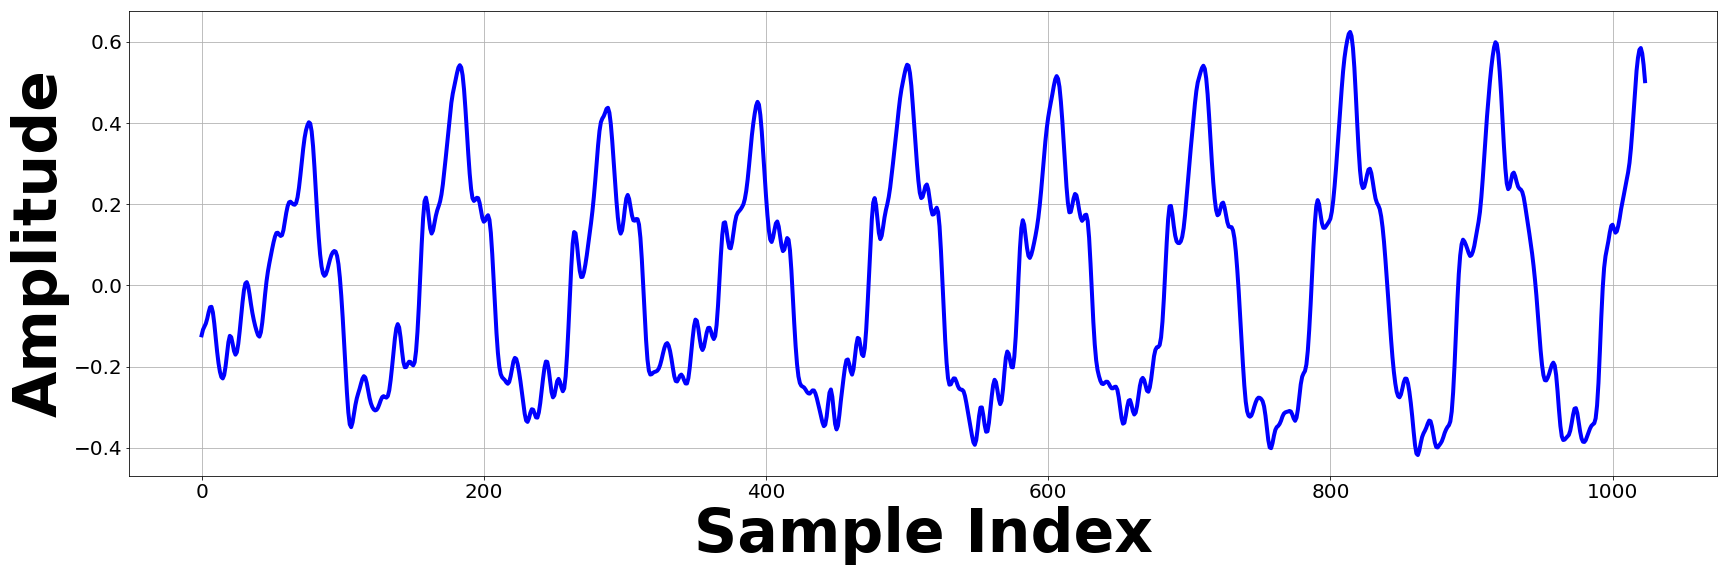
\includegraphics[width=0.45\textwidth]{figures/AnalysisFrame.png}}
    \subfigure[]{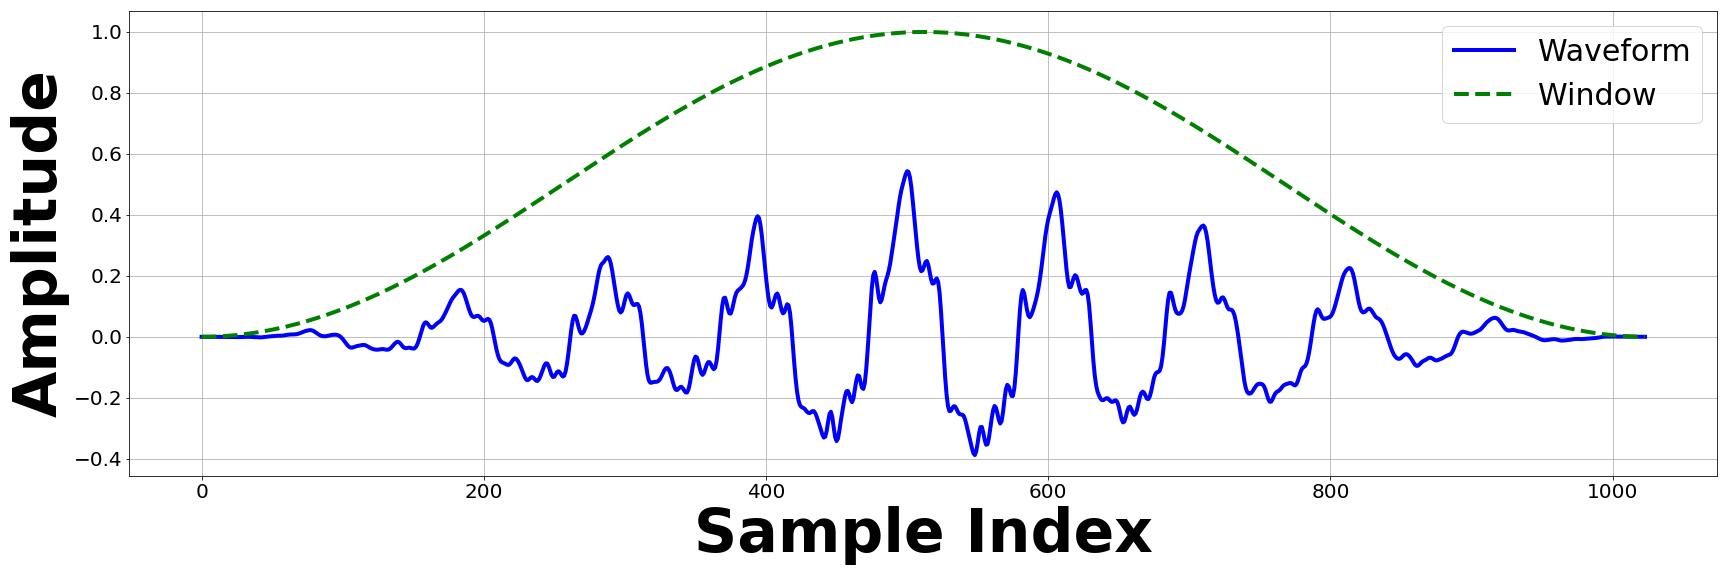
\includegraphics[width=0.45\textwidth]{figures/WindowedFrame.png}}
    \caption{(a) A standard time-series analysis frame made up of $1024$ samples and (b) The same frame with a standard Hanning Window Applied to it. This sample is taken from a bowed violin playing an $A4$ note.}
    \label{fig:WindowFrame}
\end{figure}

The standard western concert musical instruments that make up our base data set rarely have fundamental frequencies that extend beyond $6,000$ Hz. This means, that we will rarely see much energy or characteristic behavior above the $12,000$ Hz mark in the spectrograms. For this reason, we choose to crop each matrix as to include only information corresponding to the region of frequency-space form $0$ Hz to $12$ kHz. We also choose to zero pad, or crop matrix $S$ so that there are exactly $k = 256$ columns. The result is an image-like representation of a digital audio file with shape $558 \times 256$, which is passed as a feature to the input of the CNN branch of the HNN. This is the second of the two modalities that we choose to represent our data sample.

\begin{figure}[h]
    \centering
    \subfigure[]{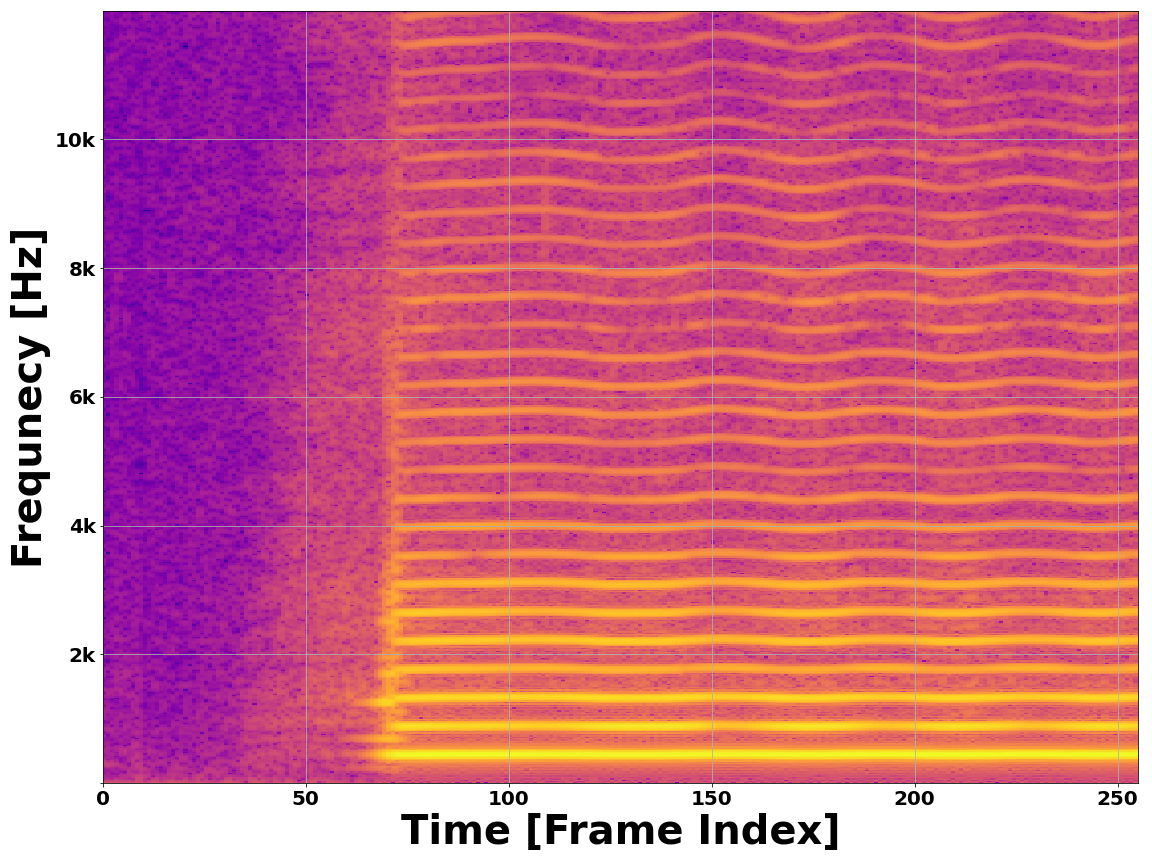
\includegraphics[width=0.45\textwidth]{figuresSpectrograms/AltoSax-A4.png}}
    \subfigure[]{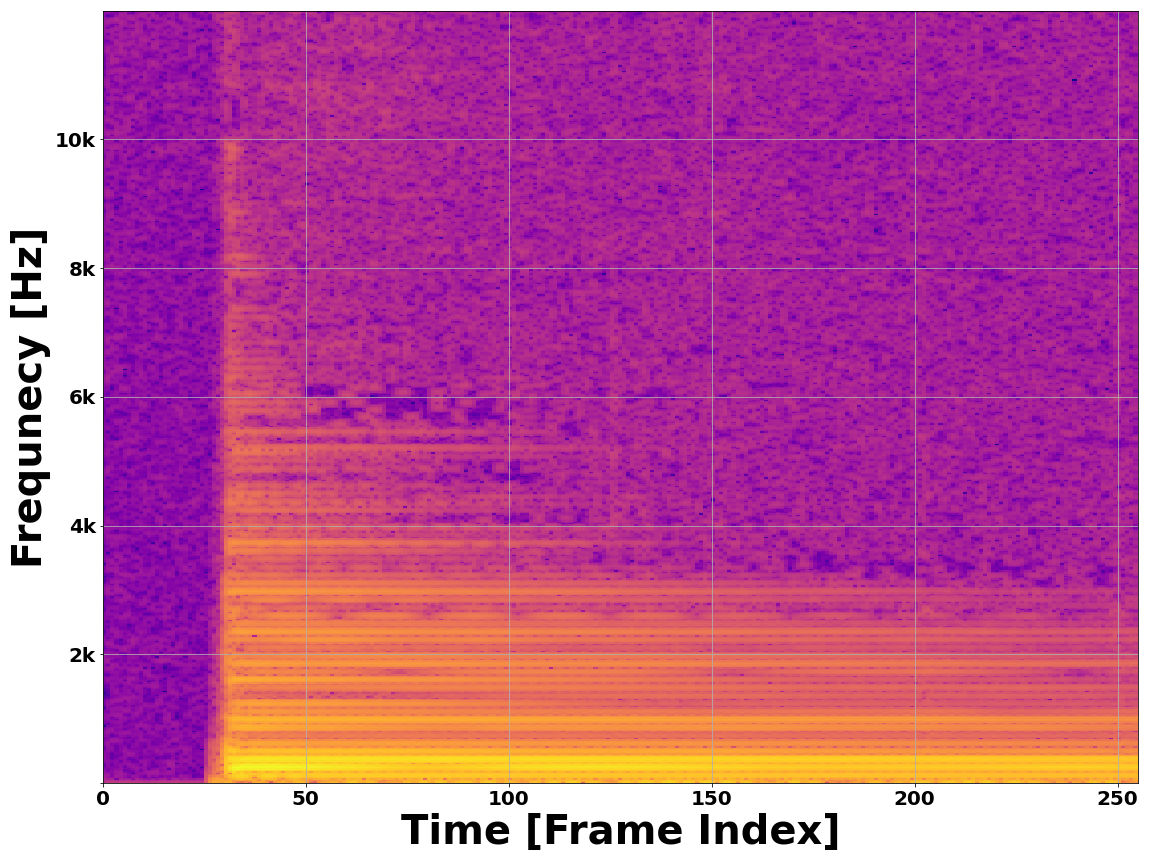
\includegraphics[width=0.45\textwidth]{figuresSpectrograms/GUITAR-B2.png}}
    \caption{Spectrograms of (a) an alto saxophone playing an $A4$ and (b) an acoustic guitar playing a $B2$}
    \label{fig:Example Spectrograms}
\end{figure}

% ================================================================

\subsection{The Perceptron Branch}
\label{subsec:MLP}

The perceptron branch is an pictured on the left side of Fig. (\ref{fig:Architecture}) and is an implementation of multilayer perceptron (MLP) neural network. The MLP processed input by transforming activations through repeated layers of neurons, modeled as vectors of floating-point numbers. Each neurons in a given layer by a linear combination of every neuron in the previous layer. Practical implementations introduce the addition of a constant value to each neuron (called a \textit{bias}), and some form or non-linear activation function \cite{Geron,Goodfellow}. Transformations of this type are called \textit{dense} layers, which when compounded can model that highly non-linear decision boundaries than arise in real world problems \cite{James}.

The input to this branch is a vector of features, described in section (\ref{subsec:FeaturesMLP}), which are transformed through two dense layers, with $64$ neurons each. Passing through these dense layers allows these inputs to be handled just like any other multilayer perceptron model, which have shown experimental success in the last few decades. We choose to implement one here, enabling the training process to learn parameters that can effectively minimize the cost function and sucessfully classify inputs. The output of the last dense layer is provided to the concatenation layer, which merges it with the output of the convolution branch. 

% ================================================================

\subsection{The Convolution Branch}
\label{subsec:CNN}

The Convolution branch is pictured on the left side of Fig. (\ref{fig:Architecture}) and is an implementation of a convolutional neural network (CNN), connected to a multilayer perceptron (MLP). This branch accepts 2D image-like input in the form of a spectrogram, described in section (\ref{subsec:FeaturesCNN}). The order and organization of the layers in this branch of the model was inspired from Oxford's \textit{VGG-16} network architecture \cite{Geron}. VGG-16 model uses successive 2D convolutions to identify characteristic features, followed by 2D pooling layers to reduce the size of the activations. Unlike VGG-16, our model does not use padding to keep the image resolution after each convolution layer, and instead the resolution of the image is dropeed with every layer.

The dominant structure in our convolution branch is the \textit{convolution layer group} with combines three layers in succession:
\begin{enumerate}
    \item \textbf{2D Convolution Layer} - $32$ features feature maps, $3 \times 3$ kernel size, $1 \times 1$ kernel stride, ReLU activation function.
    \item \textbf{2D Convolution Layer} - $32$ features feature maps, $3 \times 3$ kernel size, $1 \times 1$ kernel stride, ReLU activation function.
    \item \textbf{2D Maximum Pooling Layer} - $3 \times 3$ kernel size, $1 \times 1$ kernel stride, Identity activation function
\end{enumerate}
The combination of layers in this order allows for the convolutions to detect characteristic features in the spectrogram, while the pooling allows for minor positional in variance in those features. Additionally, the output of the layer group is smaller is size, causing each layer's activation to take up less memory, and allowing only the most prolific features of each input to survive. At the end of the final layer group, the remaining 2D image contain only a few pixels, and the activation are flattened, by reorganizing each sample such that it is a 1D array. The 1D array is appropriately shaped for processing in the branche own MLP structure. The output of the last dense layer of this MLP is provided to the concatenation layer, which merges it with the output of the Perceptron branch. 

% ================================================================

\subsection{Multirepresentation Learning}
\label{subsec:Multimodal}


\begin{figure}[h]
    \centering
    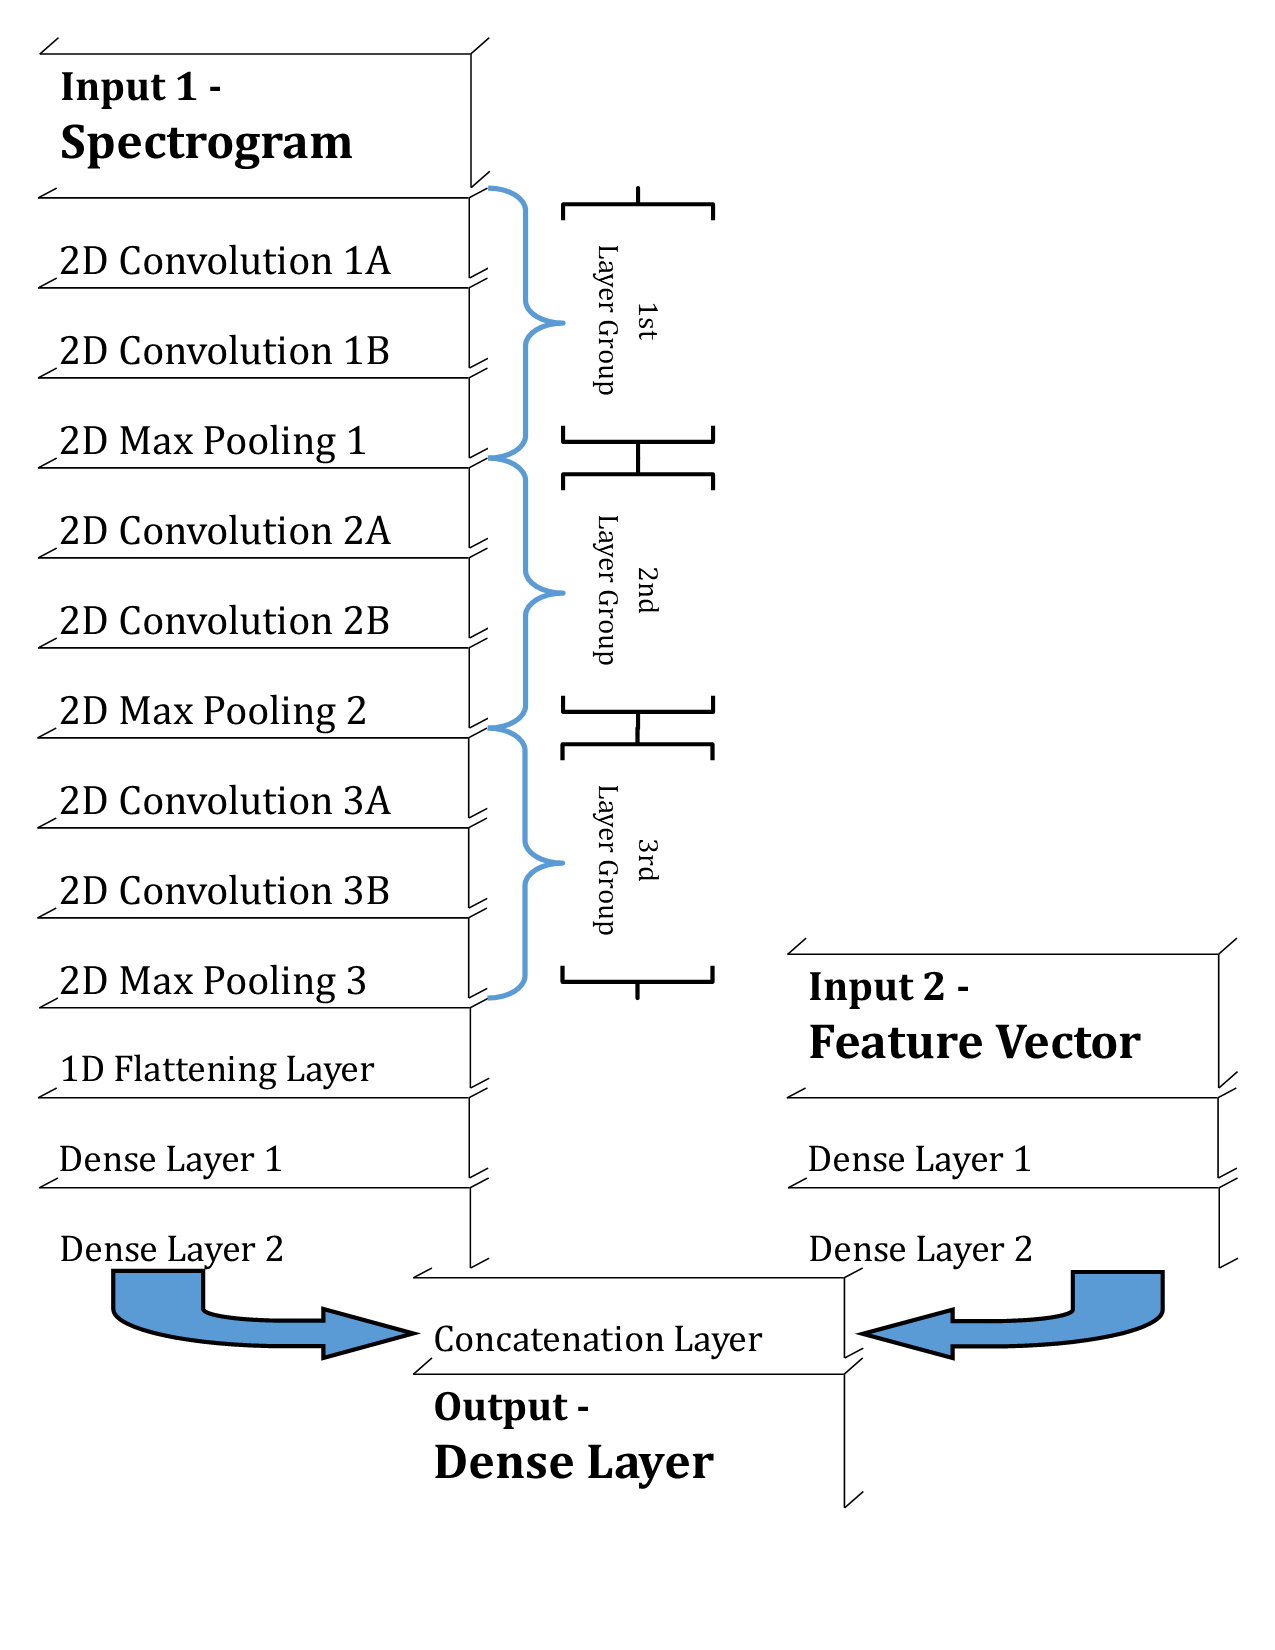
\includegraphics[width=0.45\textwidth]{figures/NeuralNetworkArchitecture.png}
    \caption{Architecture for Hybrid Neural Network model, implemented with Tensorflow \cite{Tensorflow}}
    \label{fig:Architecture}
\end{figure}

The architecture of the HNN enables us to perform classify the contents of digital audio files as musical instruments through \textit{multimodal} learning. The combined architecture, using Google's \textit{Tensorflow} library for Python allows the model to be trained conveniently as a single object \cite{Tensorflow}. This means that although the HNN is composed of two separate branches, all parameters and layers in the network are included with each back-propagation pass. This HNN contains 319,365 trainable parameters.

% ================================================================================================================================

\section{Experimental Results}
\label{sec:Results}

% ================================================================

\subsection{Resampling}
\label{subsec:Resampling}

In the machine learning workflow, it is standard practice to divide a full data set into a \textit{training} subset and a \textit{testing} subset \cite{James,Virtanen}. The training subset is used to optimize the parameters, $\Theta$, in the model as to minimize the cost function, $J$, for the data set. The testing subset is used to evaluate how well the neural network performs on data that it has never interacted with \cite{Geron}. The training subset does contain corresponding labels, but they are withheld from the trained model such that it can make unbiased predictions.
We can expand this idea to a common resampling method called \textit{K-Folds Cross Validation}, or X-validation for short \cite{James}. X-validation divides a data set into $K$ equally-sized folds. The first $K-1$ folds are used to train the model, and the last fold is used to evaluate how well the network performs on unseen samples. This process repeats of all $K$ folds.

The result of X-validation is $K$ neural network models that have all been trained and evaluated on overlapping subsets of the full data set. Each model contains a set of learned parameters, $\Theta$ that represent a possible outcome if trained on the given data set \cite{James}. By repeating this and comparing the performance across each fold, we understand how the chosen architecture and hyper-parameters influence the stability of the performance of the network. Across each fold, we expect to observe a reasonably high, as well as consistent performance. This is indicates a model that can train effectively, and generalize appropriately. X-validation is critical to ensuring that a model is behaving as expected.

% ================================================================

\subsection{Performance Metrics}
\label{subsec:Metrics}

We choose the following metrics to evaluate the performance of our HNN. All metrics are define in relation to \textit{true-positive} (TP), \textit{true-negative} (TN), \textit{false-positive} (FP), and \textit{false-negative} (FN) predictions \cite{Geron,James}. These metrics are computed for each of $K$ cross validation folds. We visualize the results of each split in Fig.(\ref{fig:XvalScores}.

\begin{itemize}
    \item \textbf{Accuracy Score} - is the ratio of correct predictions to total predictions made by the model. While accuracy is convenient for quick estimates of performance, it does not provide much statistical information on the nature of predictions made of the model. This is especially true when classes have non-uniform representations in the data set. The accuracy score of a classification algorithm is given by:
    \begin{equation}
        \text{Accuracy} = \frac{TP + FN}{TP + TN + FP + FN}
    \end{equation}
    Accuracy is bound between $0$ and $1$ with a higher score indicating better performance.
    
    \item \textbf{Precision Score} - is the ratio of correctly identified elements, to all relevant elements in the data set. The higher the score, the \textit{specific} a model is to a particular category. The precision score of a classification algorithm is given by:
    \begin{equation}
        \text{Precision} = \frac{TP}{TP + FP}
    \end{equation}
    This metric determines how many of the selected items are relevant to the problem and is bound between $0$ and $1$ with a higher score indicating better performance.
    
    \item \textbf{Recall Score} - is the ratio of correctly identified elements, to all relevant elements in the data set. The higher the score, the \textit{sensitive} a model is to a particular category. The recall score of a classification algorithm is given by:
    \begin{equation}
        \text{Recall} = \frac{TP}{TP + FN}
    \end{equation}
    This metric determines how many of the relevant items have been selected and is bound between $0$ and $1$ with a higher score indicating better performance.
    
    \item \textbf{F1 Score} - is the harmonic mean of the precision and recall scores. The higher the score, the more sensitive and specific a model is to a particular category. A high score indicate a model with both high precision and recall values. The $F1$ of a classification algorithm is given by:
    \begin{equation}
        F1 = 2 \times \frac{\text{Precision} \times \text{Recall}}{\text{Precision} + \text{Recall}}
    \end{equation}
    $F1$ score is bound between $0$ and $1$ with a higher score indicating better performance.
\end{itemize}

% ================================================================

\subsection{Confusion Matrices}
\label{subsec:Confusion}

A confusion matrix is a square array that counts the number of times a sample was predicted to be in a given class. For a $k$-categories classifier, the confusion matrix, $C$ has shape $k \times k$ where $C[i,j]$ is the number of times a sample known to be in class $i$ was predicted to be in class $j$ \cite{Geron}. A value added to the main-diagonal indicates a \textit{correct} classification, while a value on the off-diagonal indicates an \textit{incorrect} classification. We expect a well-performing classifier model to produce a diagonally-dominant confusion matrix.

A standard confusion matrix does not account for any non-uniformity in the number of samples in each class in the data set. To combat this, we divide the entries of each row of the confusion matrix by the sum of that row. This has the effect of "normalizing" the confusion matrix according to how often class appears in a data set. Just like the metrics in section (\ref{subsec:Metrics}), we construct the confusion matrix for each fold of cross validation, and then normalize it according to class occurrence. We average the $K$ matrices together and visualize the result in Fig. (\ref{fig:ConfScores}).


% ================================================================

\subsection{Cross Validation Results}
\label{subsec:Results}

We have chosen to run a $K = 10$ fold cross validation program on our model, and compute the value of the each of the four metrics described in section (\ref{subsec:Metrics}). We have also run X-validation on two similar models that represent either mode of the network. The first variant uses just a 2D spectrogram input, fed through an identical CNN + MLP as shown on the left of Fig. (\ref{fig:Architecture}). The activations are passed directly to the output layer where a prediction is made using this mode alone. Similarly, the second variant uses just a 1D feature-vector input, fed through an identical MLP as shown on the right side of Fig.(\ref{fig:Architecture}). The activations bypass the concatenation layer, and are passed directly to the output layer where a prediction is made using this mode alone. This allows us to produce an approximate comparison of how the HNN compares to the CNN or MLP models individually. Cross validation was performed on each model using a different set of random splits from the same data set. The reported scores are averged over all samples in each training data subset.

\begin{figure}[H]
    \centering
    \subfigure[]{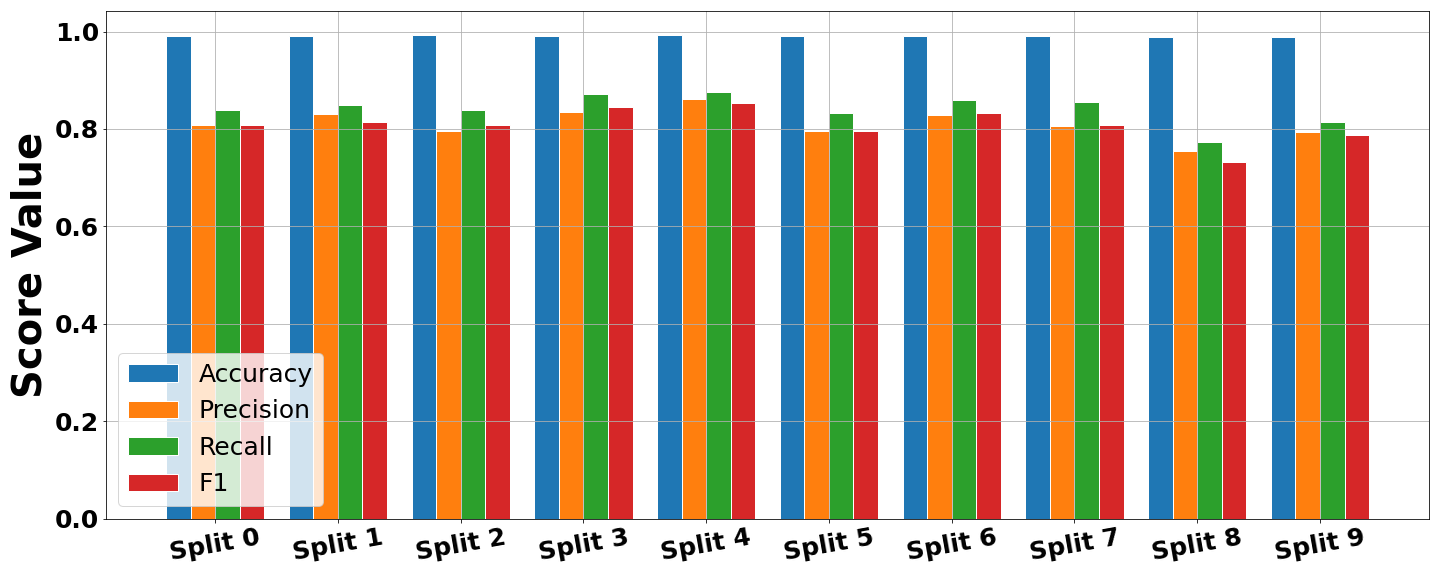
\includegraphics[width=0.45\textwidth]{figures/AvgXval-Convolution.png}}
    \subfigure[]{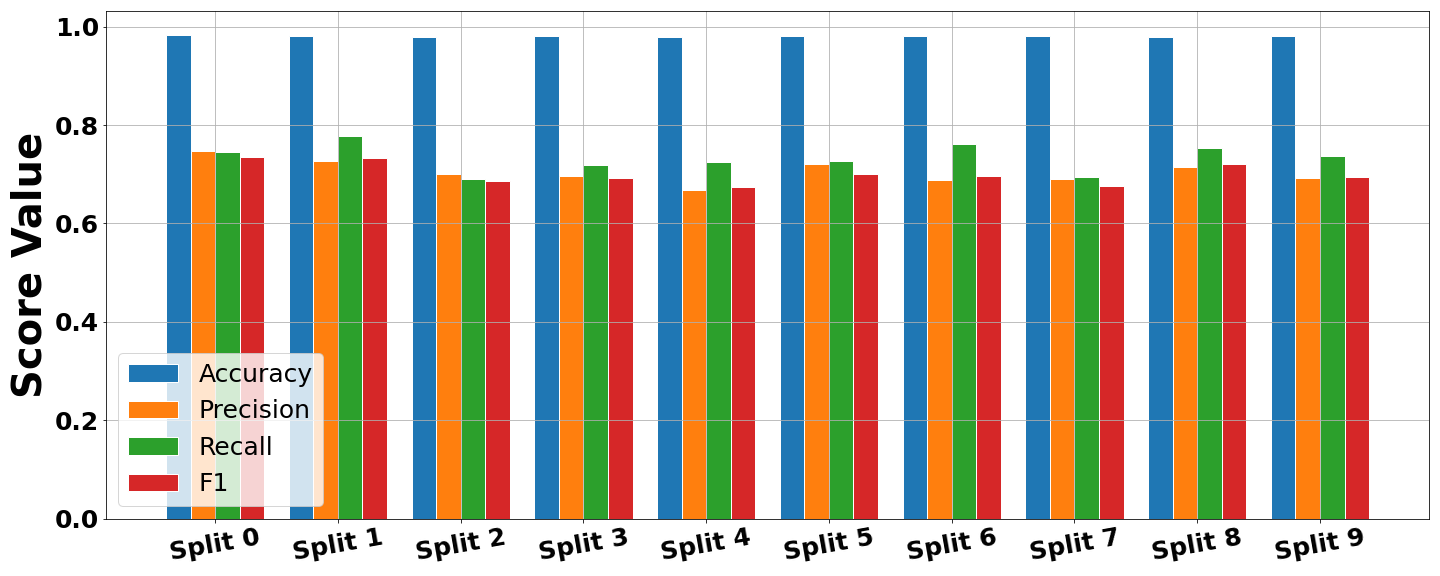
\includegraphics[width=0.45\textwidth]{figures/AvgXval-Perceptron.png}}
    \subfigure[]{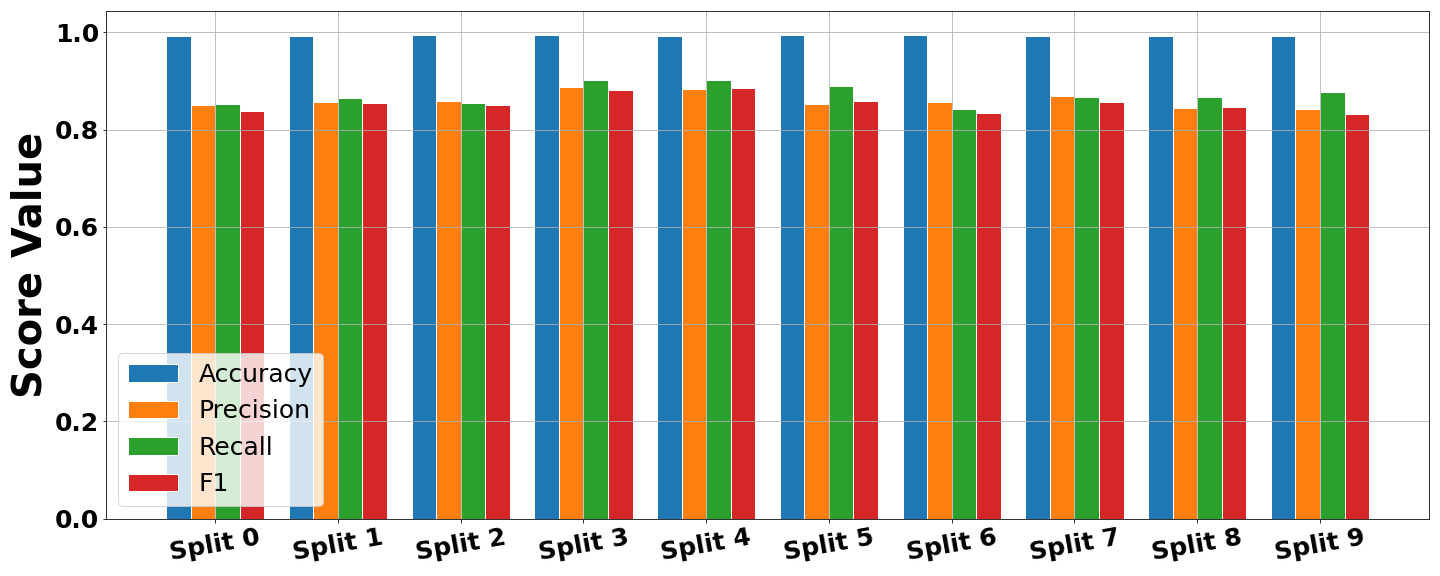
\includegraphics[width=0.45\textwidth]{figures/AvgXval-Multimodal.png}}
    \caption{Performances of the (a) CNN + MLP with spectrogram input, (b) MLP with feature-vector input, and (c) the HNN with spectrogram and feature-vector input}
    \label{fig:XvalScores}
\end{figure}

We observe the classification scores for each of the three model variants in Fig. (\ref{fig:XvalScores}). The CNN + MLP variant in (\ref{fig:XvalScores}-a) shows metric scores consistently averaging close to $0.8$. with a few splits above or below this value. Similarly, the MLP variant in (\ref{fig:XvalScores}-b) shows scores all consistently close to $0.7$.  This indicates that each input mode and complementary architecture allows for the optimization of a set of parameters to enable reasonable classification performance on unseen samples. Both models do exhibit fluctuation in the range of scores between each fold, which indicates that each model is vulnerable to small changes in initial conditions. 

The HNN architecture variant in (\ref{fig:XvalScores}-c) shows improved performance when compared to either the CNN or MLP variant alone. Where the single input mode models shows performance scores averaging around $0.8$ and $0.7$, in (\ref{fig:XvalScores}-a) and (\ref{fig:XvalScores}-b) respectivly, the HNN boasts a higher average, around $0.84$ for both precision and recall. We also observe a lower variance between the performances of each split, indicating a more stable architecture that is less susceptible to changes in initial condition. 

We also choose to examine and compare the normalized confusion matrices of the three modal variants. In Fig. (\ref{fig:ConfScores}-a) we see a confusion matrix for the CNN + MLP, which shows a strong main diagonal, indicated by the dark reds, oranges, and yellows which indicated a high-level of correct classifications. We do observe indexes such as $C[0,5]$, $C[0,15]$, $C[7,27]$, and $C[28,24]$ that contain unusually large entries indicated by the bright blue color. In Fig. (\ref{fig:ConfScores}-b) we see a weaker diagonally dominant matrix for the MLP, which displayed even more misclassified samples, spread through the matrix. Note how each confusion matrix represents the average of $10$ confusion matrices produced from cross validation. 

Finally, we observe the normalized confusion matrix of the HNN model in Fig. (\ref{fig:ConfScores}-c). This matrix is the most-diagonally dominant, showing only a few commonly confused classes. The smaller number of mis-classifications in this model indicates a greater performance, and a generally stronger classifier. We observe $C[0,15]$, $C[7,27]$, and $C[27,7]$ to have unusually large entries also indicated by the bright blue pixels. Consulting the list of instrument classes reveals that class $0$ and $15$ represent \textit{alto flutes} and \textit{flutes} respectively.  Classes $7$ and $27$ represents \textit{bass trombones} and \textit{tenor trombones}. These pairs of instruments are similar in build and in timbre, meaning that they likely have similar properties in feature space, and that a human listener may also show difficulty differentiating them. 



% ================================================================

\subsection{Practical Example}
\label{subsec:Example}

As a practical demonstration of the classification ability of the Hybrid Neural Network, we choose to test the model on an unlabeled digital audio file, "\textit{zcombo.wav}". This audio file contains a waveform that is generated through 

\textcolor{red}{I'll need your help to introduce the chaotic Synth files, and address how they are generated, and why we use and "care" about them}

\begin{figure}[H]
    \centering
    \subfigure[]{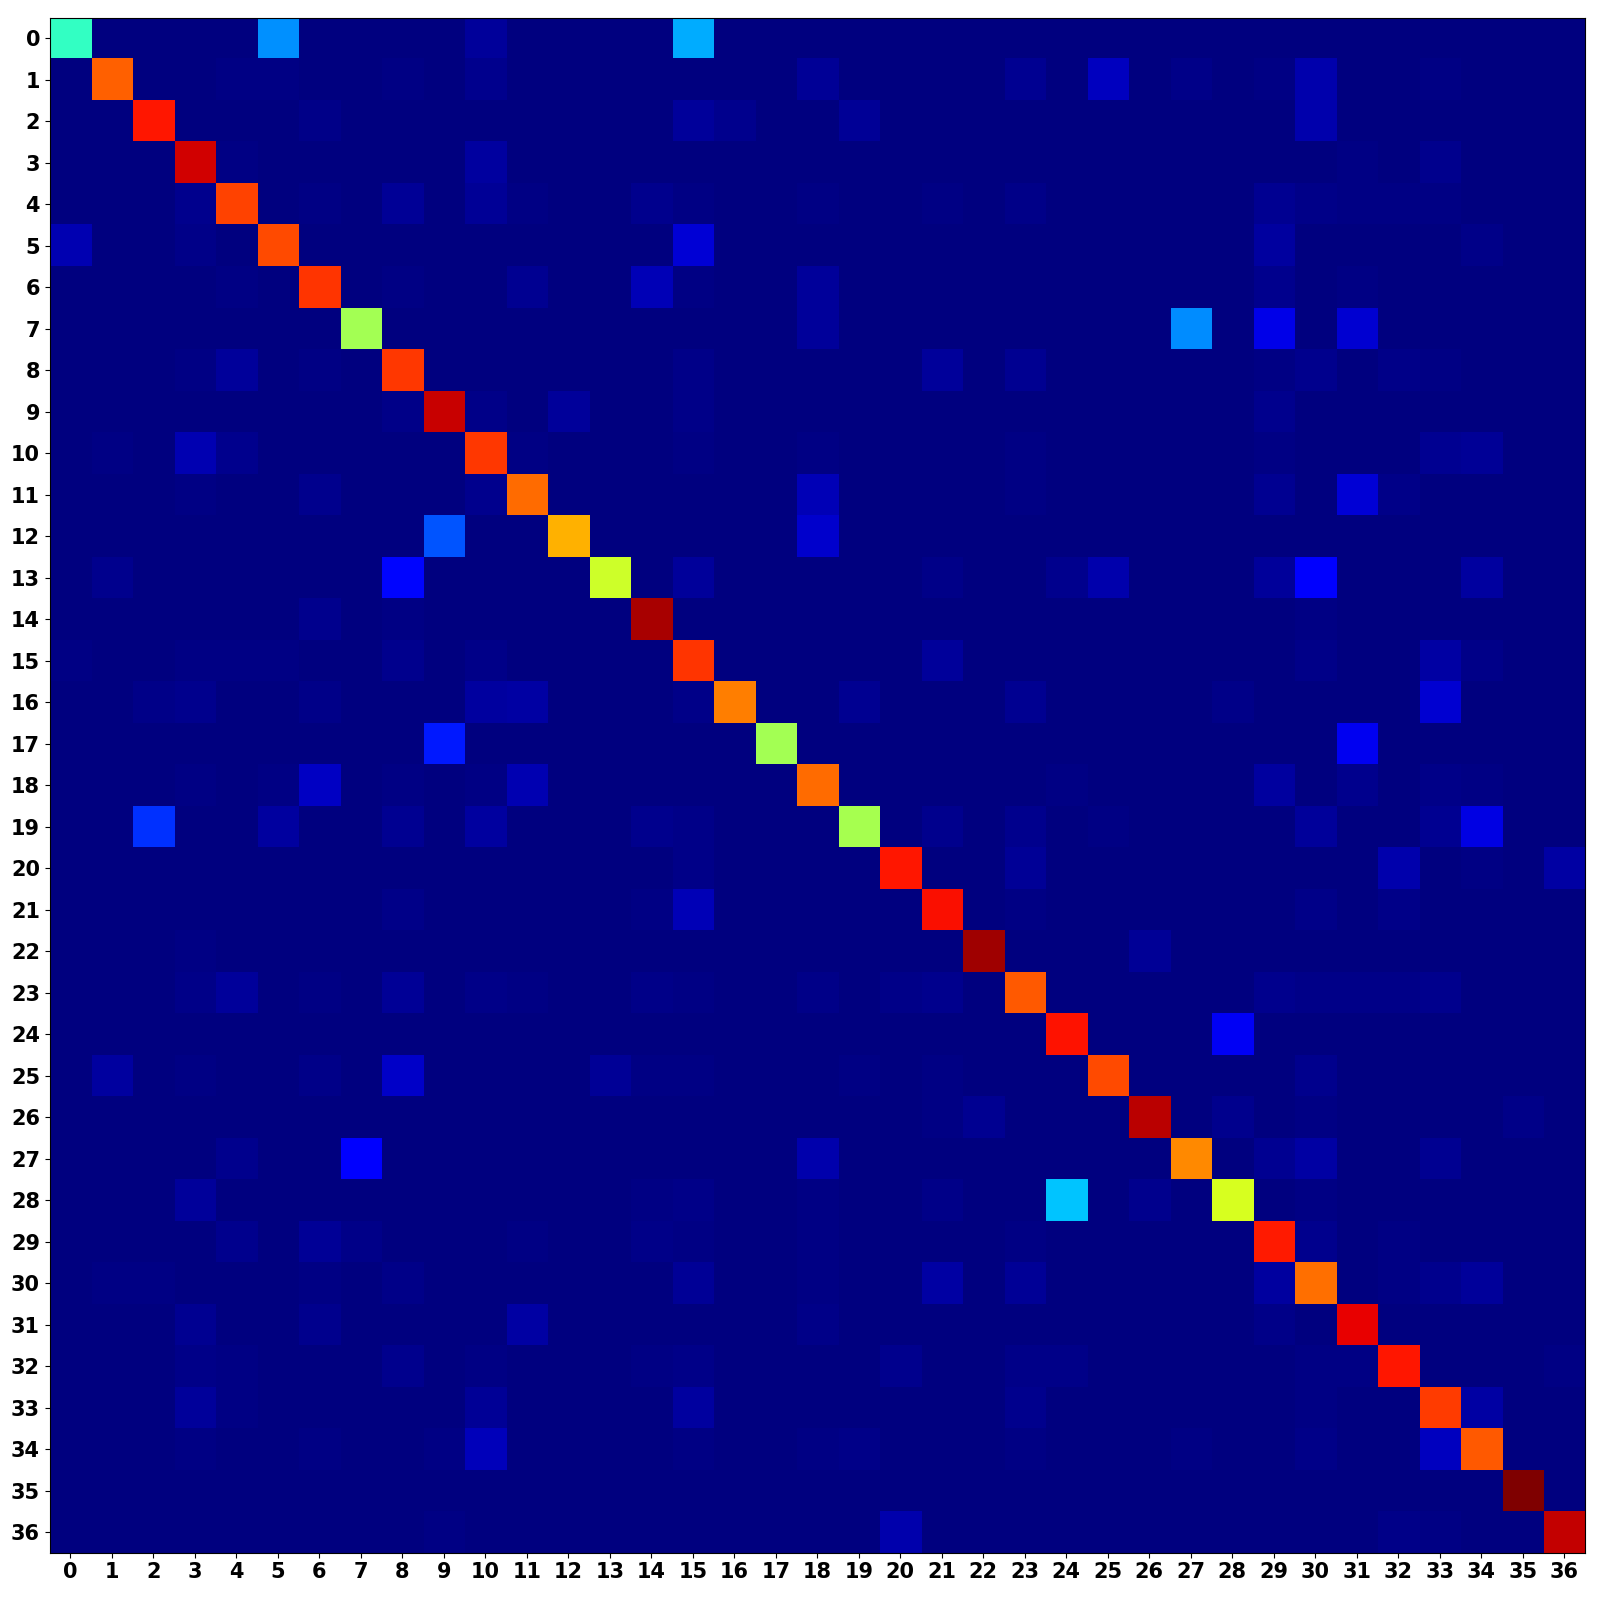
\includegraphics[width=0.35\textwidth]{figures/XValGammaCNN_Avg_Hits_Weighted_Confusion.png}}
    \subfigure[]{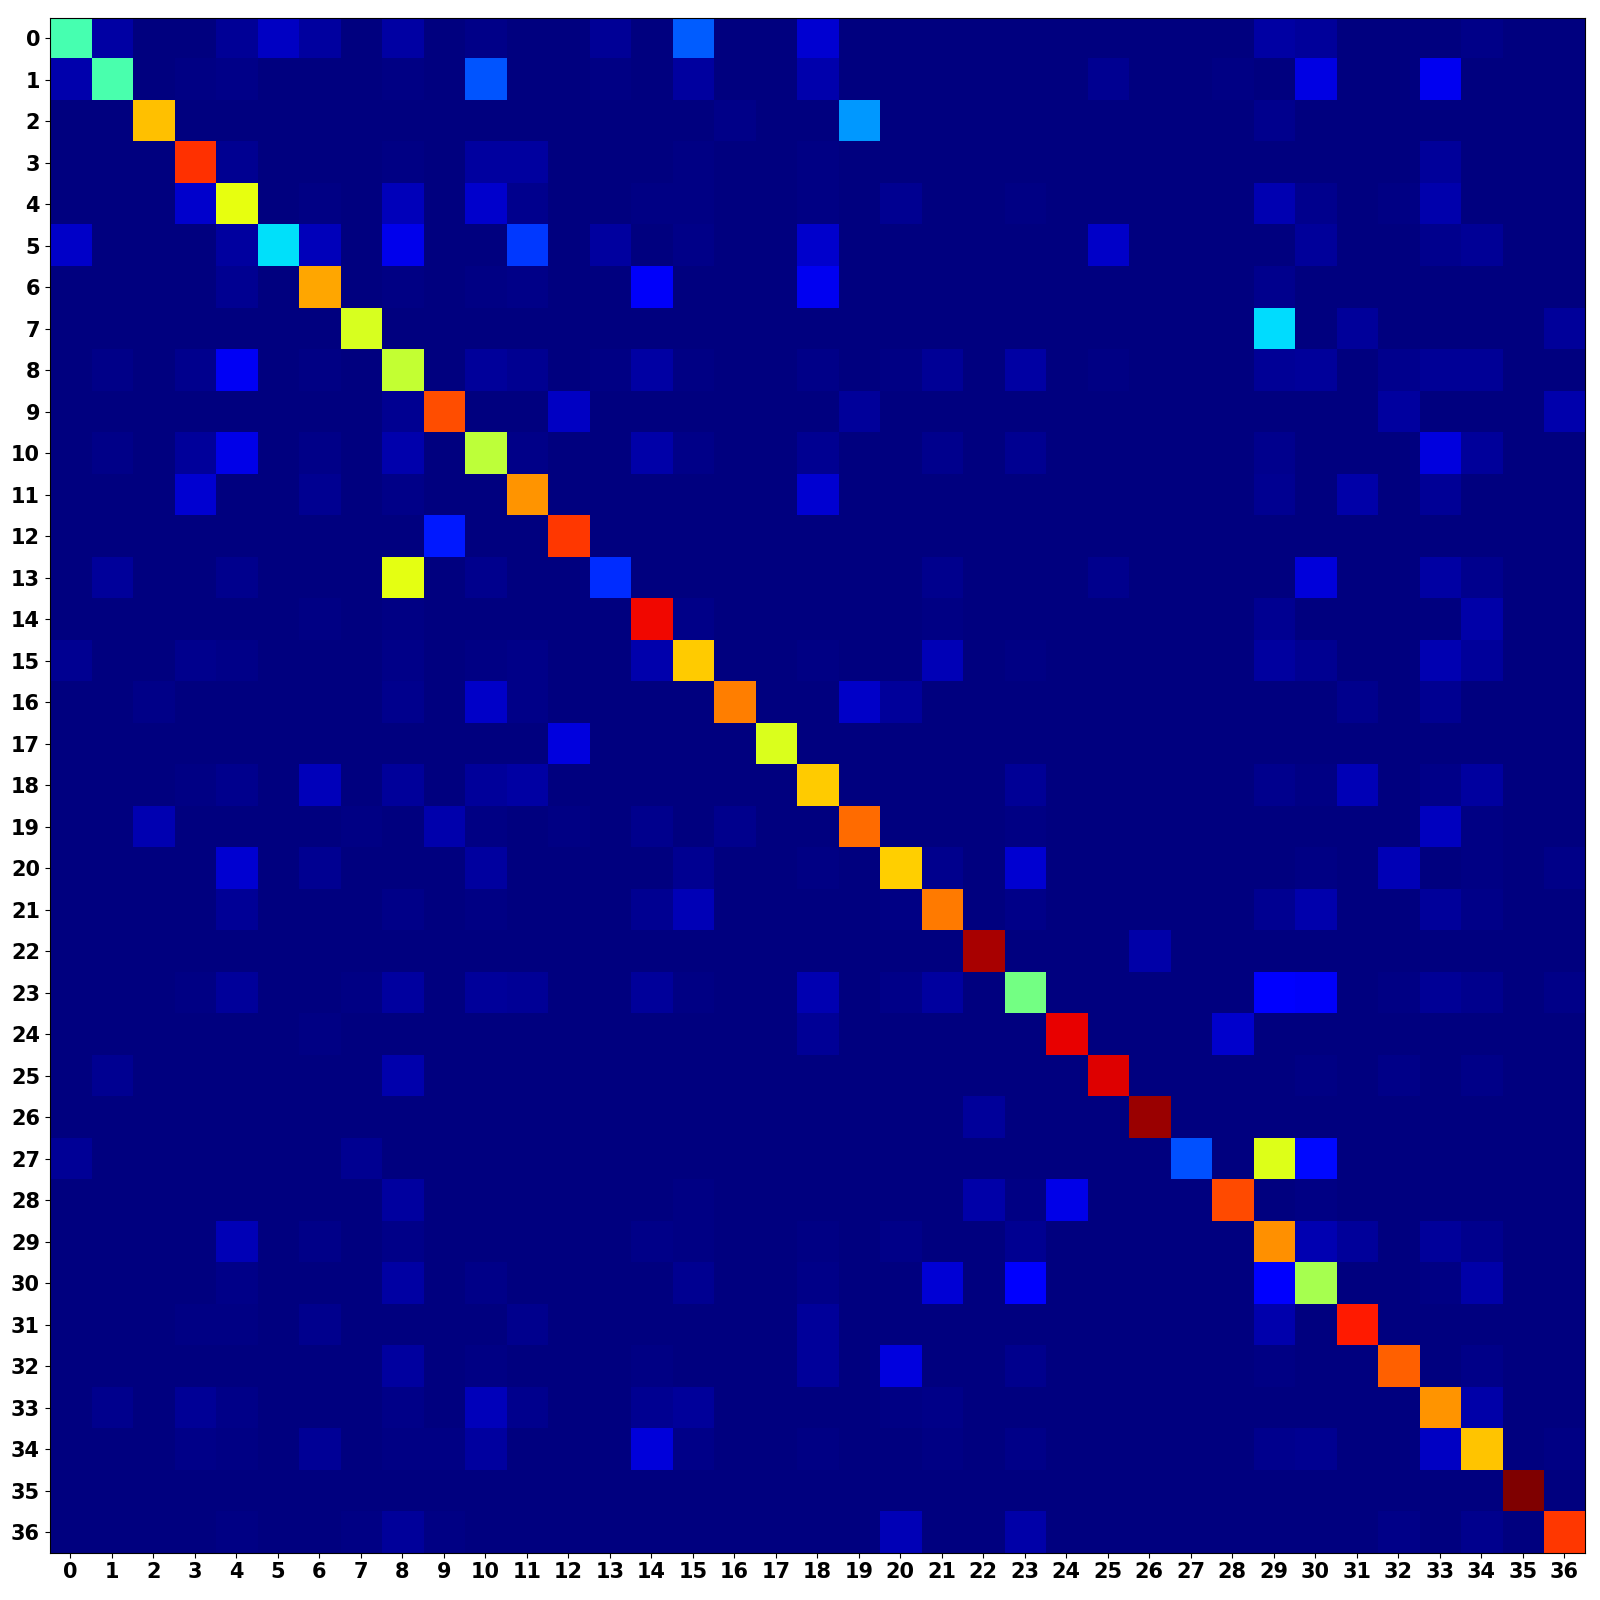
\includegraphics[width=0.35\textwidth]{figures/XValBetaMLP_Avg_Hits_Weighted_Confusion.png}}
    \subfigure[]{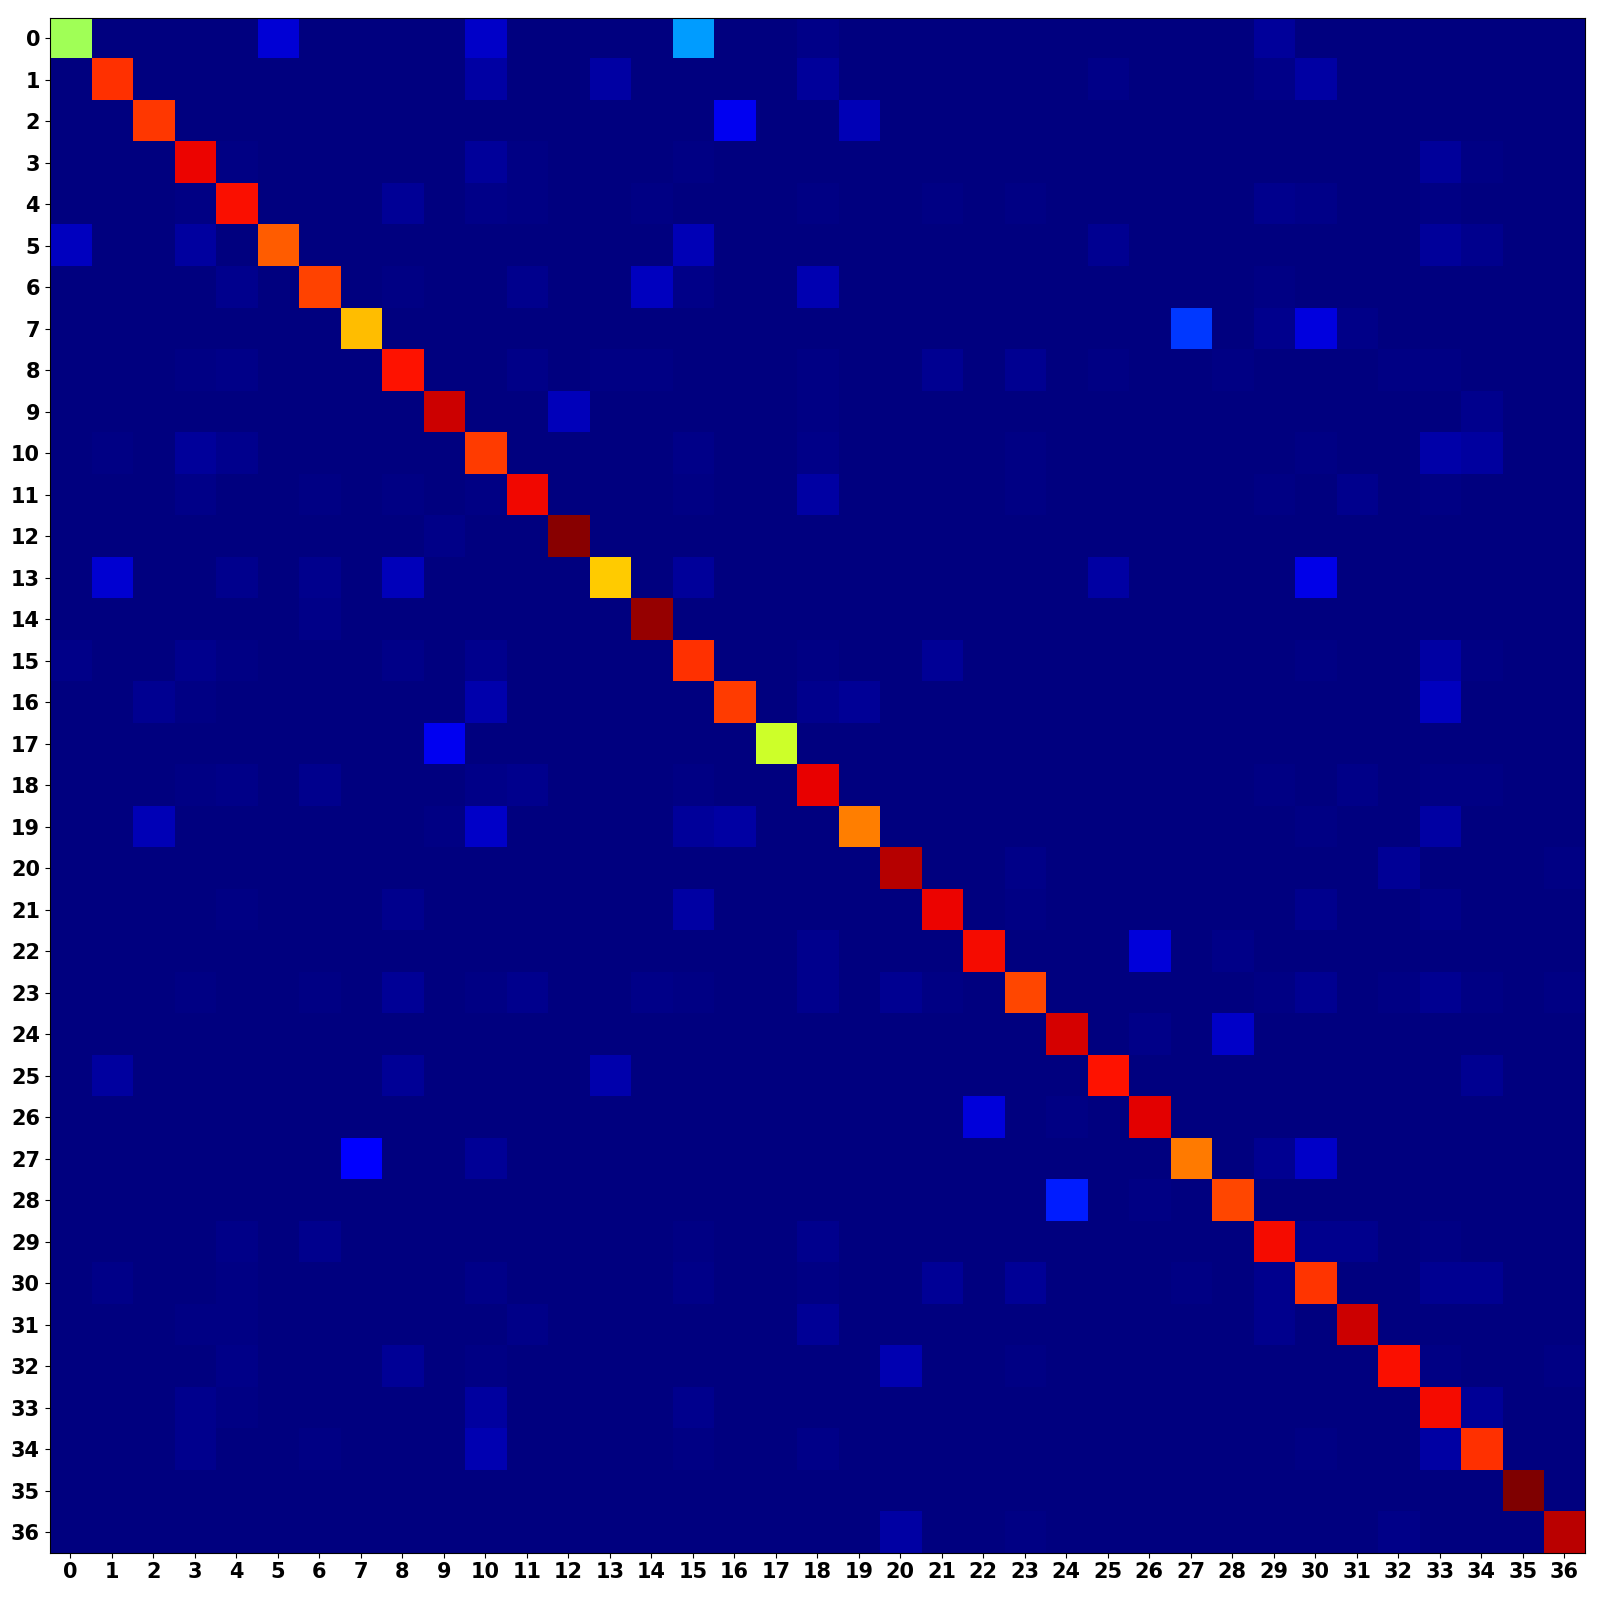
\includegraphics[width=0.35\textwidth]{figures/XValAlphaCLF_Avg_Hits_Weighted_Confusion.png}}
    \caption{Performances of the (a) CNN + MLP with spectrogram input, (b) MLP with feature-vector input, and (c) the HNN with spectrogram and feature-vector input}
    \label{fig:ConfScores}
\end{figure}

% ================================================================================================================================

\section{Discussion and Conclusion}
\label{sec:conclusion}

Multimodal learning itself shows great promise to machine learning algorithms in numerous domains. For data sets that lend themselves to multiple representations of a single sample, the ability to use those different modes allows for a more comprehensive representation of data. Across full data set, this will enable a model to generate a more stable set of parameters for classification which has the potential to yield better performance. Multimodal learning does not limit itself to classification of digital audio, but instead opens the door to many genres of machine learning such a medicine, finance, and other media classification.
 
The results of cross validation indicate that we have constructed a hybrid neural network that accept two input modes, and can effectivly classify the contents of a digital audio file as one of $37$ different musial instruments. The design of this HNN enables the input of two non-compatible modal representations of a sample to be processed and combined to form a single output prediction. We find that this model demonstrates better and more consistent performance at musical instrumental classification when compared to that of either the constituent CNN or MLP models. By transforming each input sample into multiple representations of itself, the HNN learns a more robust set of parameters that can more thoroughly differentiate each class. While some common misclassfications are present, many of them are due to the related nature of musical instruments, which may also cause similar confusion in human listeners. 

\textcolor{red}{I sure cannot write a conclusion to save my life}



% ================================================================================================================================

\begin{thebibliography}{9}

\bibitem{Geron}
Geron, Aurelien. \textit{Hands-on Machine Learning with Scikit-Learn and TensorFlow: Concepts, Tools, and Techniques to Build Intelligent Systems}. O'Reilly, 2017.

\bibitem{Goodfellow}
Goodfellow, Ian, et al.\textit{Deep Learning}. MIT Press, 2017.

\bibitem{James}
James, Gareth, et al. An Introduction to Statistical Learning with Applications in R. Springer, 2017

\bibitem{Khan}
Khan, M. Kashif Saeed, and Wasfi G. Al-Khatib. “Machine-Learning Based Classification of Speech and Music.” Multimedia Systems, vol. 12, no. 1, 2006, pp. 55–67., doi:10.1007/s00530-006-0034-0.

\bibitem{Levine}
Levine, Daniel S. Introduction to Neural and Cognitive Modeling. 2nd ed., Routledge, 2000.

\bibitem{Li}
Li, Yingming, and Ming Yang. “A Survey of Multi-View Representation Learning.” Journal of LateX Class Files, vol. 14, no. 8, Aug. 2015. 

\bibitem{Liu}
Liu, Zhu, et al. "Audio Feature Extraction and Analysis for Scene Segmentation and Classification." Journal of VLSI Signal Processing, vol. 20, 1998, pp. 61–79.

\bibitem{McCulloch}
McCulloch, Warren S., and Walter Pitts. "A Logical Calculus of the Ideas Immanent in Nervous Activity." \textit{The Bulletin of Mathematical Biophysics}, vol. 5, no. 4, 1943, pp. 115–133.

\bibitem{Mierswa}
Mierswa, Ingo, and Katharina Morik. ”Automatic Feature Extraction for Classifying Audio Data.” Machine Learning, vol. 58, no. 2-3, 2005, pp. 127–149., doi:10.1007/s10994-005-5824-7.


\bibitem{Ngiam}
Ngiam, Jiquan, et al. "Multimodal Deep Learning." 2011. 

\bibitem{Philharmonia}
Philharmonia Symphony Orchestra home page- \textit{https://philharmonia.co.uk/}

\bibitem{Sahidullah}
Sahidullah, Goutam S. “Design, Analysis and Experimental Evaluation of Block Based Transformation in MFCC Computation for Speaker Recognition.” 18 Nov. 2011.

\bibitem{Tensorflow}
TensorFlow: Large-scale machine learning on heterogeneous systems,
2015. Software available from tensorflow.org.

\bibitem{Virtanen}
Virtanen, Tuomas, et al. \textit{Computational Analysis of Sound Scenes and Events.} Springer, 2018.

\bibitem{UnivIowa}
University of Iowa Electronic Music Studios home page- \textit{http://theremin.music.uiowa.edu/}

\bibitem{Zhang}
Zhang, Tong, and C.-C. Jay Kuo. “Content-Based Classification and Retrieval of Audio.” \textit{Advanced Signal Processing Algorithms, Architectures, and Implementations VIII}, 2 Oct. 1998, pp. 432–443., doi:10.1117/12.325703.

\end{thebibliography}

% ================================================================================================================================

\end{document}
